\subsection{Implementation and deployment}
\label{sec:deployment}

%\begin{figure}[t]
%  \centering
%  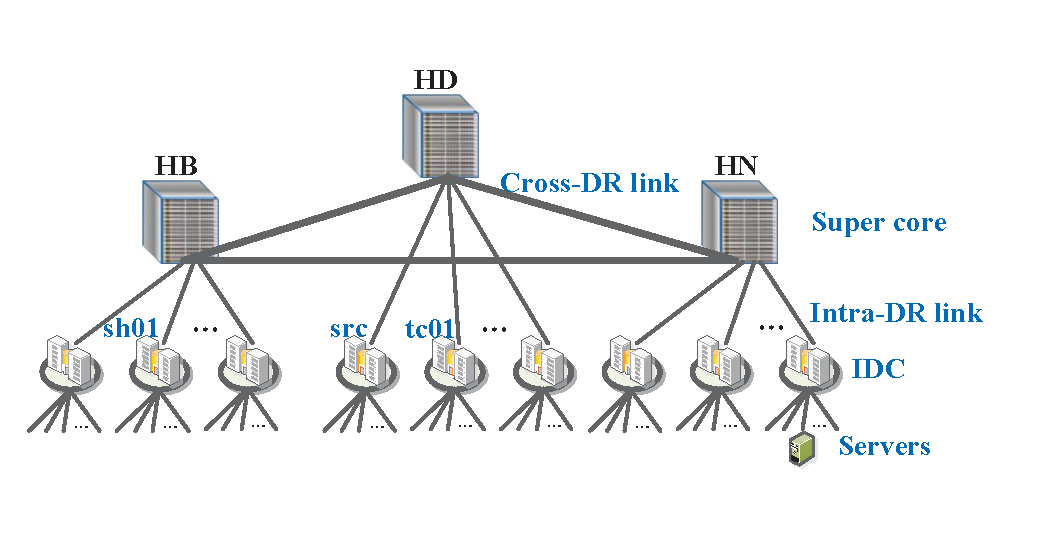
\includegraphics[width=3in]{images/Testbed_v2.eps}
%  \tightcaption{The abstract topology of our intra-net WAN.}
%  \label{fig:topology}
%\vspace{-0.1in}
%\end{figure}
%\vspace{-15pt}

We have deployed \name on \company's DCs, which consist of 67 geo-distributed servers in 10 DCs. Evaluation in the next section is based on this deployment. %The topology is shown as Fig. \ref{fig:topology}.

\name is implemented with 3621 lines of golang code \cite{golang}, and it was fully integrated in \company's DCs. The duplications of the controller are implemented on three different geo-located zookeeper servers.
The data plane bulk data transmissions between controller and agents use TCP, and the control plane decision messages use \texttt{HTTP POST}. For specific transmissions, \name uses \texttt{wget} to make data transfer, and enforce bandwidth by \texttt{--limit-rate}.
%\jc{add linux tc stuff here}
The agent running in each server uses Linux Traffic Control (\texttt{tc}) to enforce the limit on the total bandwidth usage of inter-DC multicast traffic.
%Thus, \name achieves the bandwidth separation dynamically and in real-time.

%\jc{explain the application-facing api}

 %\jc{which option?}

\name n be seamlessly integrated with applications because \name's implementation makes no specific requirements on applications. All the applications need to do is to call the public APIs provided by \name to complete three steps: first, register on \name, assign the source DC, destination DCs, servers and the bulk data; second, install agents on all those servers; third, set the start time of bulk data transfers. Then \name will start the data distribution at the specified time. Such simple implementation also makes \name applicable to other companies' DCs. 	

%\jc{this is oversimplistic. did you make any assumption about the agent? what if a hadoop application wants to use your stuff?}

%\jc{a missing piece is what's application interface. if an application wants to send a file, does it make a function call to your system?}

%\jc{what changes did you make on each server? where was the controller implemented? what's the protocol? how did data transfer happen (wget?)? how was bandwidth enforcement done (wget option)? }



%
%\begin{itemize}
%\item \name consists of \fillme line of \fillme code, and can be fully integrated in \company's DCs.
%
%\item Application interfaces: What information does an application need to announce to \name to initiate a multicast.
%
%\item What's the software platform to implement each component
%
%\item Why \name is also applicable to other DCs?
%
%\end{itemize}

